\section{Evaluation}
\label{evaluation}

In this section, we evaluate Spatial by comparing programmer productivity and the performance of generated designs to Xilinx's commercial HLS tool, SDAccel. We then evaluate the HyperMapper design tuning approach and demonstrate Spatial's advantages for portability across FPGAs and the Plasticine CGRA.


\subsection{FPGA Performance and Productivity}
We first evaluate the FPGA performance and productivity benefits of Spatial against SDAccel, a commercial C-based programming tool from Xilinx for creating high-performance accelerator designs. We use SDAccel in our study as it has similar performance and productivity goals as Spatial, supports the popular OpenCL programming model, and performs several optimizations related to loop pipelining, unrolling, and memory partitioning~\cite{sdaccel}. Baseline implementations of the benchmarks in Table~\ref{t:hls_comp} have been either obtained from a public SDAccel benchmark suite from Xilinx~\cite{sdaccelBench}, or written by hand. Each baseline has then been manually tuned by using appropriate HLS pragmas~\cite{hlsPragmaRef} to pick loop pipelining, unrolling, and array banking factors, and to enable dataflow optimizations. Design points for Spatial are chosen using the DSE flow described in Section~\ref{dse}.

We measure productivity by comparing number of lines of source code used to describe the FPGA kernel, excluding host code. We measure performance by comparing runtimes and FPGA resources utilized for each benchmark on a Xilinx Ultrascale+ VU9P board with a fabric clock of 125 MHz, hosted on an Amazon EC2 F1 instance. We generate FPGA bitstreams targeting the VU9P architecture for each benchmark using both Spatial and SDAccel, and obtain resource utilization data from the post place-and-route reports. We then run and verify both designs on the FPGA and measure the execution times on the board. CPU setup code and data transfer time between CPU and FPGA is excluded from runtime measurements for both tools.

Table~\ref{t:hls_comp} shows the input dataset sizes and the full comparison between lines of source code, resource utilization, and runtime of the benchmarks implemented in SDAccel and Spatial.
In terms of productivity, language constructs in Spatial like \texttt{\small{load}} and \texttt{\small{store}} for transferring dense sparse data from DRAM reduces code bloat and increases readability.
Furthermore, by implicitly
inferring parameters such as parallelization factors and loop initiation intervals, Spatial code is largely free of annotations and pragmas.

Spatial achieves speedups over SDAccel of $1.63\times$ and $1.33\times$ respectively on \emph{BlackScholes} and \emph{TPC-H Q6}. Both benchmarks
stream data from DRAM through a deeply pipelined datapath which is amenable to FPGA acceleration. Dataflow support in SDAccel using the DATAFLOW pragma~\cite{dataflowRef} and streaming support in Spatial allows both tools to efficiently accelerate such workloads. In \emph{K-Means}, coarse-grained pipelining support allows Spatial to achieve roughly the same performance as SDAccel using $1.5\times$ fewer BRAMs.
Specialized DRAM scatter/gather support enables Spatial to achieve a $3.48\times$ speedup on \emph{PageRank}.

We see speedups of $8.48\times$, $1.37\times$, and $14.15\times$ for compute-heavy workloads \emph{GDA}, \emph{GEMM}, and \emph{SW}, respectively. The baseline for \emph{SW} is implemented by Xilinx as a systolic array, while the Spatial implementation uses nested controllers. \emph{GEMM} and \emph{GDA} contain opportunities for coarse-grained pipelining that are exploited within Spatial. 
GDA, for example, contains an outer product operation, during which the data in the same buffer is repeatedly accessed and reused. While this operation can be pipelined with a preceding loop producing the array, SDAccel's DATAFLOW pragma does not support such access patterns that involve reuse. As a result, SDAccel requires larger array partitioning and loop unrolling factors to offset the performance impact, at the expense of consuming more FPGA BRAM.
In addition, nested controllers in \emph{GEMM}
can be parallelized and pipelined independently in Spatial, while SDAccel automatically unrolls all inner loops if an outer loop is parallelized. Spatial can therefore explore
design points that cannot be easily expressed in SDAccel. Finally, as the Spatial compiler performs analyses on a parameterized IR, the compiler can reason about larger parallelization factors without expanding the IR graph.
SDAccel unrolls the graph as a preprocessing step, hence creating larger graphs when unrolling and array partitioning factors are large.
This has a significant impact on the compiler's memory footprint and compilation times, making better designs difficult or impossible to find.

Spatial provides a productive platform to program FPGAs, with a 42\% reduction in lines of code compared to SDAccel averaged across all benchmarks. On the studied benchmarks, Spatial achieves a geometric mean speedup of $2.9\times$ compared to an industrial HLS tool.



\subsection{Design Space Exploration}


% We next evaluate the efficiency of HyperMapper for quickly approximating Pareto frontier over two design objectives: design runtime and FPGA logic utilization (LUTs).
% For this evaluation, we run HyperMapper with 1000 initial random samples and run 5 subsequent active learning iterations of at most 100 samples each. In comparison, heuristic search prunes using the same heuristics as defined in the DHDL work~\cite{dhdl} and then randomly samples up to 100,000 points. We perform 10 trials for both design space exploration approaches.

% Figure~\ref{figHVI} shows the hypervolume indicator (HVI) as a function of design tuning time, averaged across trials, for two representative benchmarks, \emph{K-Means} and \emph{GDA}. 
% The HVI gives the area difference between the Pareto frontier found at a given point in time compared to the best Pareto curve computed across all trials of both approaches.
% For applications with medium sized design spaces like \emph{K-Means}, HyperMapper is able to reach the same accuracy as the heuristic approach within about the same exploration time, and is able to find better points when run for twice as long. This is because HyperMapper is driven by active learning, enabling effective design space exploration without pruning potentially good points.
% On larger spaces like \emph{GDA}'s, HyperMapper's performance is limited by the presence of invalid design points which can not fit on to the target FPGA in the design space. 
% Since HyperMapper currently does not account for design point validity, it spends much of its time searching an invalid portion of the space, and consequently has a lower accuracy than randomized search. In future work, we plan to evaluate the addition of valid design prediction to HyperMapper on the accuracy of estimated Pareto curves.

% \begin{figure}
% \centering
% %%% trim = left, bottom, right, top
% \begin{subfigure}[t]{0.48\linewidth}
% \includegraphics[clip, trim=0.0cm 0.0cm 0.0cm 2.85cm, width=\linewidth]{figs/Kmeans_hvi.pdf}
% \caption{K-Means}
% \end{subfigure}
% ~
% \begin{subfigure}[t]{0.48\linewidth}
% \includegraphics[clip, trim=0.0cm 0.0cm 0.0cm 2.85cm, width=\linewidth]{figs/GDA_hvi.pdf}
% \caption{GDA}
% \end{subfigure}

% \vspace{-10pt}
% \caption{HVI (Pareto accuracy) for HyperMapper and heuristic DSE approaches over design tuning time. The 95\% confidence interval is shown by the shaded area. \vspace{-10pt}}
% \label{figHVI}
% \end{figure}


We next perform a preliminary evaluation of HyperMapper for quickly approximating Pareto frontier over two design objectives: design runtime and FPGA logic utilization (LUTs).
For this evaluation, we run HyperMapper with several seeds of initial random sample, with the number of samples $R$ ranging from 1 to 6000 designs, and run 5 active learning iterations of at most 100 samples each. For comparison, the heuristic search proposed in the DHDL work~\cite{dhdl} prunes using simple heuristics and then randomly samples up to 100,000 points. For both approaches, design tuning takes up to 1 -- 2 minutes, varying slightly by benchmark complexity.

Figure~\ref{hvi_samples} shows the hypervolume indicator (HVI) function
for the \emph{BlackScholes} benchmark as a function of the initial
number of random samples.
The HVI gives the area between the estimated Pareto frontier and the space's true Pareto curve, found from exhaustive search.
By increasing
the number of random samples to bootstrap the active learning phase,
we see two orders
of magnitude improvement in HVI. Furthermore, the overall variance goes down very
quickly as the number of random
samples increases. As a result, the autotuner is robust
to randomness and only a handful of random samples are
needed to bootstrap the active learning phase. As shown in Figure~\ref{paretos},
HyperMapper is able to reach a close approximation of
the true Pareto frontier with less than 1500 design points.

On benchmarks like GDA with sparser design spaces, HyperMapper spends much of its time evaluating areas 
of the space with invalid designs which cannot fit on the FPGA.
HyperMapper's accuracy for these benchmarks is consequently lower than the heuristic approach.
Consequently, in future work, we plan to extend HyperMapper with a valid design prediction mechanism and evaluate this tuning approach on a wider class of benchmarks.

% \begin{figure}
% \centering
% \vspace{-10pt}
% \caption{HyperMapper's HVI (Pareto accuracy) versus number of initial random samples. \vspace{-20pt}}
% \label{figHVI}
% \end{figure}


\begin{figure}
\centering
%%% trim = left, bottom, right, top
\begin{subfigure}[t]{0.45\linewidth}
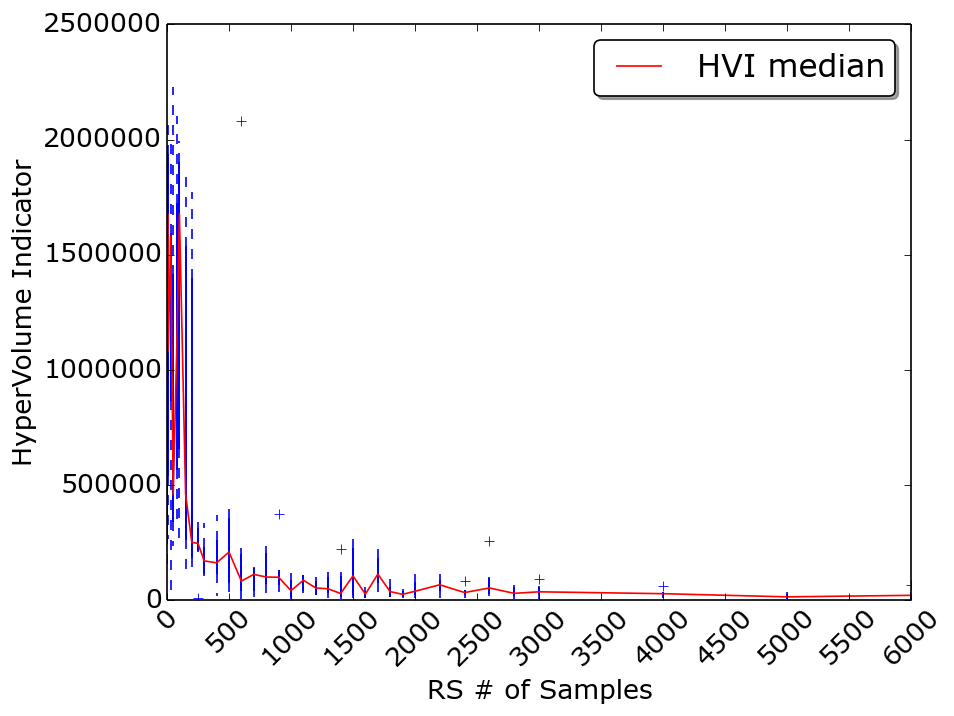
\includegraphics[width=\linewidth]{images/DSE/hvi_5NumberSummary_median.png}
\subcaption{HyperMapper HVI versus initial random samples ($R$) five number summary.}
\label{hvi_samples}
\end{subfigure}\hspace{15pt}
~
\begin{subfigure}[t]{0.45\linewidth}
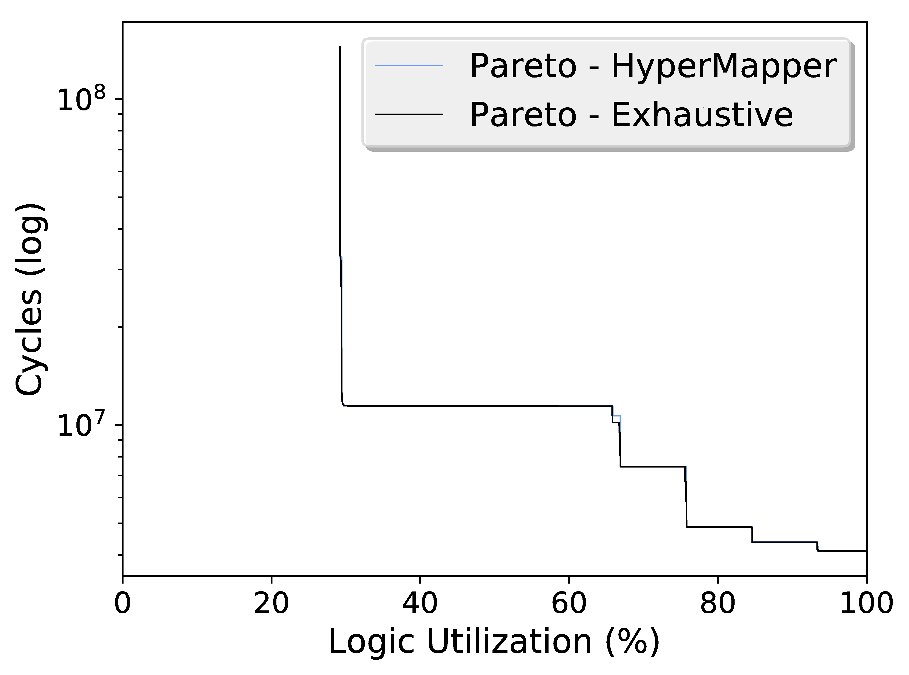
\includegraphics[clip, trim=0.0cm 0.0cm 0.0cm 0.0cm, width=\linewidth]{figs/output_pareto_blackscholes.pdf}
\subcaption{Exhaustive and HyperMapper ($R$=1000) generated Pareto curves. }
\label{paretos}
\end{subfigure}

\vspace{-10pt}
\caption{Design space tuning on \emph{BlackScholes}.}
\label{figHVI}
\end{figure}

% \begin{table}[ht]
% \centering
% \caption{Runtime to reach accuracy of TODO\% and corresponding variance for design tuning with heuristic search and HyperMapper.\vspace{-10pt}}
% \label{tableDSE}

% \fontsize{7}{9}\selectfont
% \begin{tabular}{llrrrrr}
%                       & \multicolumn{2}{c}{\textbf{Space Size}} & \multicolumn{2}{c}{\textbf{Heuristic}} & \multicolumn{2}{c}{\textbf{HyperMapper}} \\
%                       & \mc{Total} & \mc{Pruned}    & \mc{Time} & \mc{Var}  &   \mc{Time} & \mc{Var} \\ \midrule
%   %\bf{Dot Product}   & 117,964,800      & 1,085,952            &              &                &                &               \\ \midrule  
%   %\bf{Outer Product} & 16,588,800       & 31,068               &              &                &                &               \\ \midrule
%   \bf{BS}             & 7.7$\times 10^4$  & 6.7$\times 10^2$    &              &                &                &               \\ \midrule
%   \bf{GDA}            & 3.0$\times 10^{10}$ & 4.6$\times 10^6$  &              &                &                &               \\ \midrule
%   \bf{GEMM}           & 2.6$\times 10^8$  & 1.4$\times 10^5$   &              &                &                &               \\ \midrule
%   \bf{KMeans}         & 2.1$\times 10^6$  & 1.9$\times 10^4$   &              &                &                &               \\ \midrule
%   \bf{SW}             & 2.1$\times 10^6$  & 3.3$\times 10^4$   &              &                &                &               \\ \midrule
%   \bf{TQ6}            & 3.5$\times 10^9$  & 2.3$\times 10^6$   &              &                &                &               \\ \bottomrule
% \end{tabular}
% \end{table}


\subsection{Spatial Portability}

\begin{table}
\centering
\caption{Runtimes (ms) of tuned designs on ZC706, followed by runtimes and speedup~($\times$) of directly porting these designs to the VU9P, then runtimes and successive speedup over ported designs when tuned for the VU9P. The \emph{Total} column shows the cumulative speedup. \vspace{-5pt} }
\label{fig:zynq_comp}

\centering
\fontsize{7}{9}\selectfont
\begin{tabular}{l d{2.1} d{2.1} d{2.1} d{2.1} d{2.1} d{2.1}}
   \bf{FPGA}      & \mc{ZC706}  & \multicolumn{4}{c}{\bf VU9P}                                       & \mc{Total}     \\ 
   \bf{Design}    & \mc{Tuned}  & \multicolumn{2}{c}{\bf Ported}   & \multicolumn{2}{c}{\bf Tuned}    &               \\ \toprule

                  & \mc{Time}   & \mc{Time}  & \mc{$\times$}       & \mc{Time}  & \mc{$\times$}       & \mc{$\times$} \\ \midrule
   \ml{BS}        & 89.0        & 35.6       & 2.5                 & 3.8        & 9.4                 & 23.4          \\ \midrule
   \ml{GDA}       &  8.4        & 3.4        & 2.5                 & 1.3        & 2.6                 & 6.5           \\ \midrule
   \ml{GEMM}      & 2226.5      & 1832.6     & 1.2                 & 878.5      & 2.1                 & 2.5           \\ \midrule
   \ml{KMeans}    & 358.4       & 143.4      & 2.5                 & 53.3       & 2.7                 & 6.7           \\ \midrule
   \ml{PageRank}  & 1299.5      & 1003.3     & 1.3                 & 587.4      & 1.7                 & 2.2           \\ \midrule
   \ml{SW$^\dag$} & 1.3         &  0.5       & 2.5                 & 0.5        & 1.0                 & 2.5           \\ \midrule
   \ml{TQ6}       & 69.4        & 15.0       & 4.6                 & 14.0       & 1.1                 & 5.0           \\ \bottomrule
   
   \multicolumn{7}{l}{\vspace{10pt}\footnotesize{ $^\dag$SW with 160 base pairs, the largest to fit on the ZC706.}}
\end{tabular}
\vspace{-10pt}
\end{table}

We next demonstrate the portability of Spatial code by targeting two different FPGA architectures; (1) the Zynq ZC706 SoC board, and (2) The Virtex Ultrascale+ VU9P on the Amazon EC2 F1.
Designs on the VU9P use a single DRAM channel with a peak bandwidth of 19.2 GB/s. The ZC706 is much smaller than the VU9P in terms of FPGA resource and has a smaller DRAM bandwidth of 4.26 GB/s.
We target both the ZC706 and VU9P from the same Spatial code for all benchmarks listed in Table~\ref{t:hls_comp}. Benchmarks are tuned for each target using
target-specific models with automated DSE. Clock frequency is fixed at 125 MHz for both FPGAs. 

Table~\ref{fig:zynq_comp} shows the speedups achieved on the VU9P over the ZC706. The results show that not only can the same Spatial source code be ported
to architectures with different capabilities, the application can also be automatically tuned to better take advantage of resources in each target.
Compute-bound benchmarks \emph{BlackScholes}, \emph{GDA}, \emph{GEMM}, \emph{K-Means} achieve speedups of up to $23\times$ on the VU9P over the ZC706. Porting these designs to the VU9P alone has a $1.2\times$ to $2.5\times$ due to increased main memory bandwidth, but a majority of the benefit of the larger FPGA comes from tuning the parallelization factors to use more resources. 
While \emph{SW} is also compute bound, the size of the dataset was limited by the smaller FPGA. In this case, the larger capacity of the VU9P does not improve runtime, but instead allows handling of larger datasets. 

Memory-bound benchmark \emph{TPC-H Q6} benefits from the higher DRAM bandwidth available on the VU9P. Porting this benchmark immediately gives a $4.6\times$ runtime improvement from the larger main memory bandwidth, while further parallelizing controllers to create more parallel address streams to DRAM helps the application make better use of this bandwidth. \emph{PageRank} is also bandwidth-bound, but the primary benefit on the VU9P comes from specializing the memory controller to maximize utilized bandwidth for sparse accesses.


% \begin{table}
% \caption{Speedup of VU9P over ZC706. \vspace{-10pt} }
% \label{fig:zynq_comp}

% \fontsize{8}{10}\selectfont
% \begin{tabular}{cccccc} 
% \bf{GDA}     & \bf{GEMM}    & \bf{K-Means} & \bf{PageRank} & \bf{SW}      & \bf{TQ6} \\ \hline
% 2.54$\times$ & 2.53$\times$ & 1.84$\times$ & 2.21$\times$  & 1.74$\times$ & 4.97$\times$  \\ \hline
% \end{tabular}
% \end{table}




\begin{table}
\centering
\caption{Plasticine DRAM bandwidth, resource utilization, runtime, and speedup ($\times$) over VU9P FPGA. \vspace{-5pt} }
\label{table:plasticine_eval}

\centering
\fontsize{7}{7}\selectfont
\resizebox{0.99\columnwidth}{!}{
  \begin{tabular}{m{0.5cm} d{2.1} d{2.1} d{2.1} d{2.1} d{2.1} d{2.1} r }
  \toprule
                 & \multicolumn{2}{c}{\bf Avg DRAM } & \multicolumn{3}{c}{\bf Resource }        & \mc{}     & \mc{} \\
                 & \multicolumn{2}{c}{\bf BW (\%)}   & \multicolumn{3}{c}{\bf Utilization (\%)} & \mc{Time} & \mc{$\times$} \\
   \bf{App}     & \mc{Load}    & \mc{Store} & \mc{PCU}  & \mc{PMU}  & \mc{AG}   & \mc{(ms)} & \mc{} \\ \midrule
   \ml{BS}       & 77.4        & 12.9       & \mb{\hspace{1pt}73.4} & 10.9      & 20.6      & 2.33      & 1.6   \\
   \ml{GDA}      & 24.0        & 0.2        & \mb{\hspace{1pt}95.3} & 73.4      & 38.2      & 0.13      & 9.8   \\
   \ml{GEMM}     & 20.5        & 2.1        & \mb{\hspace{1pt}96.8} & 64.1      & 11.7      & 15.98     & 55.0  \\
   \ml{KMeans}   & 8.0         & 0.4        & \mb{\hspace{1pt}89.1} & 57.8      & 17.6      & 8.39      & 6.3   \\
   \ml{TQ6}      & \mb{\hspace{2pt}97.2}   & 0.0        & 29.7      & 37.5      & \mb{70.6} & 8.60      & 1.6   \\

\bottomrule
\end{tabular}}
\vspace{-10pt}
\end{table}


Finally, we demonstrate the portability of Spatial beyond
FPGA architectures by extending the compiler to map
the Spatial IR to target our proposed Plasticine CGRA~\cite{plasticine}. Plasticine is a
two-dimensional array of compute (PCUs) and memory
(PMUs) tiles with a statically configurable interconnect
and address generators (AG) at the periphery to perform
DRAM accesses. The Plasticine architecture is a significant departure
from an FPGA, with more constraints on memory banking and computation, including
fixed size, pipelined SIMD lanes.

We simulate Plasticine with  a $16 \times 8$ array of 64 compute and 64 memory tiles, with a 1 GHz clock and a main memory with a DDR3-1600 channel with 12.8 GB/s peak bandwidth.
Table~\ref{table:plasticine_eval} shows the DRAM bandwidth, resource utilization, runtime, and speedup of the Plasticine CGRA over the VU9P for a subset of benchmarks.

Streaming, bandwidth-bound applications like \emph{TPC-H Q6} efficiently exploit about 97\% of the available DRAM bandwidth.
Compute-bound applications \emph{GDA}, \emph{GEMM}, and \emph{K-Means} use around 90\% of Plasticine's compute tiles.
Plasticine's higher on-chip bandwidth also allows these applications to better utilize the compute resources, giving these applications speedups of $9.9\times$, $55.0\times$, and $6.3\times$.
Similarly, the deep compute pipeline in \emph{BlackScholes} occupies 73.4\% of compute resources after being split across multiple tiles, 
giving a speedup of $1.6\times$. 

%We implemented comparable versions of each of our benchmarks in C++ and synthesized them
%using HLS and SDAccel tools.  There are certain constructs in Spatial that allow
%certain algorithms to be expressed more concisely and in slightly different, but intuitive, ways that
%expose the strengths of the language.  Each application exhibits certain characteristics which 
%can be exploited by certain aspects in the programming paradigms of Spatial and HLS. Specifically,
%they can be characterized as compute-bound applications and memory-bound applications, with some
%tradeoff between the two depending on design decisions.  While HLS is the industry standard for
%exposing FPGAs to domain experts, our results show that Spatial is a suitable alternative that can
%lead to better designs for certain algorithms with less overhead.

%Spatial is a suitable platform for the designer who is interested in making the most of the
%available resources, as it allows quick design tradeoffs in the app without needing to use complex pragmas throughout the app.
%In applications that are memory bound, such as AES, BlackScholes, and Sobel, we would expect that neither
%design could acheive significantly better speedup since they have access to the same DRAM interfaces.  
%For compute-bound applications, such as Kmeans, GEMM, and GDA, there is a large, interesting design space that
%Spatial can quickly expose to the user.

%\begin{figure}
%\centering
%\includegraphics[width=1\columnwidth, trim=0.5cm 0.9cm 1.0cm 0]{figs/f1_comp.png}
%\caption{Speedup and resource utilization comparisons with SDAccel on F1.}
%\label{fig:f1_comp}
%\end{figure}

% \subsection{Portability Across FPGAs and CGRAs}
% We demonstrate the applicability of Spatial to beyond FPGA architectures by extending the compiler
% to map Spatial IR to the Plasticine CGRA~\cite{plasticine}. Plasticine is a two-dimensional array of compute (PCUs) and memory (PMUs) tiles
% with a statically configurable interconnect and address generators (AG) at the periphery to perform DRAM accesses.
% Plasticine is a significant departure from FPGA with different kinds of constraints on memory banking and parallelization.

% Similar to the FPGA, we construct area and runtime models specific to Plasticine, and drive the design space exploration to tune
% benchmarks to Plasticine. Compiling to Plasticine then involves lowering the Spatial IR to a target-specific IR for the Plasticine low-level mapping compiler,
% which outputs a configuration bitstream. Resource utilization reports are obtained from the low-level compiler.
% Execution times are measured by simulating the generated bitstream in a cycle-accurate fashion at a clock frequency of 1 GHz. 



%Fortunately, due to the locality exhibited by these applications, designs with large tile sizes that do not maximize the off-chip
%bandwidth are capable of achieving comparable performance to the ones that have 100\%
%compute unit utilization. Hence, the best performing design point shown in
%Table~\ref{table:plasticine_eval} does not correspond to the design with 100\% compute utilization.

%Therefore, the given architecture cannot fit unrolling the outer loop by more than 1 without 
%exceeding 100\% PCU utilization. 
%\todo{K-Means is a sequential iterative convergence algorithm that neither outer loop nor
%inner loop that computes the new centroids can be parallelized.} As a result, we could not maximize
%either bandwidth or resource.}

%For application that are not memory-bound, yet Plasticine is not able to take larger
%unrolling factors, such as BlackScholes and K-Means, Plasticine still achieves roughly $4-7\times$
%speedup compared to F1 due to its higher clock frequency.

%Figure~\ref{fig:gemm_dse} shows the design space of GEMM on Plasticine. The bottom edged circles are
%designs with large tile size that better capture locality. The dark large circles on the right are 
%designs with good PCU and PMU utilization, and high DRAM load bandwidth as result of outer loop
%unrolling. 



%\begin{figure}
%\centering
%\includegraphics[width=1\columnwidth]{figs/GEMM_Blocked.png}
%\caption{Design space for GEMM on Plasticine}
%\label{fig:gemm_dse}
%\end{figure}

%\begin{figure}
%\centering
%\begin{minipage}{.5\linewidth}
  %\centering
  %\includegraphics[width=1\linewidth]{reg_K-FOLD}
  %\caption{Regularization}
  %\label{fig:reg}
%\end{minipage}%
%\end{figure}
%\subsection{GEMM Case Study}
%\gist{gemm}
